\PassOptionsToPackage{unicode=true}{hyperref} % options for packages loaded elsewhere
\PassOptionsToPackage{hyphens}{url}
%
\documentclass[a4paper, notitlepage, 12pt, krantz2]{krantz}
\usepackage{lmodern}
\usepackage{amssymb,amsmath}
\usepackage{ifxetex,ifluatex}
\usepackage{fixltx2e} % provides \textsubscript
\ifnum 0\ifxetex 1\fi\ifluatex 1\fi=0 % if pdftex
  \usepackage[T1]{fontenc}
  \usepackage[utf8]{inputenc}
  \usepackage{textcomp} % provides euro and other symbols
\else % if luatex or xelatex
  \usepackage{unicode-math}
  \defaultfontfeatures{Ligatures=TeX,Scale=MatchLowercase}
\fi
% use upquote if available, for straight quotes in verbatim environments
\IfFileExists{upquote.sty}{\usepackage{upquote}}{}
% use microtype if available
\IfFileExists{microtype.sty}{%
\usepackage[]{microtype}
\UseMicrotypeSet[protrusion]{basicmath} % disable protrusion for tt fonts
}{}
\IfFileExists{parskip.sty}{%
\usepackage{parskip}
}{% else
\setlength{\parindent}{0pt}
\setlength{\parskip}{6pt plus 2pt minus 1pt}
}
\usepackage{hyperref}
\hypersetup{
            pdfauthor={Oliver Gardi, Fifonsi Dangbo, Sophie Dzigbod, Ditorgue Bakabima},
            pdfborder={0 0 0},
            breaklinks=true}
\urlstyle{same}  % don't use monospace font for urls
\usepackage{longtable,booktabs}
% Fix footnotes in tables (requires footnote package)
\IfFileExists{footnote.sty}{\usepackage{footnote}\makesavenoteenv{longtable}}{}
\usepackage{graphicx,grffile}
\makeatletter
\def\maxwidth{\ifdim\Gin@nat@width>\linewidth\linewidth\else\Gin@nat@width\fi}
\def\maxheight{\ifdim\Gin@nat@height>\textheight\textheight\else\Gin@nat@height\fi}
\makeatother
% Scale images if necessary, so that they will not overflow the page
% margins by default, and it is still possible to overwrite the defaults
% using explicit options in \includegraphics[width, height, ...]{}
\setkeys{Gin}{width=\maxwidth,height=\maxheight,keepaspectratio}
\setlength{\emergencystretch}{3em}  % prevent overfull lines
\providecommand{\tightlist}{%
  \setlength{\itemsep}{0pt}\setlength{\parskip}{0pt}}
\setcounter{secnumdepth}{5}
% Redefines (sub)paragraphs to behave more like sections
\ifx\paragraph\undefined\else
\let\oldparagraph\paragraph
\renewcommand{\paragraph}[1]{\oldparagraph{#1}\mbox{}}
\fi
\ifx\subparagraph\undefined\else
\let\oldsubparagraph\subparagraph
\renewcommand{\subparagraph}[1]{\oldsubparagraph{#1}\mbox{}}
\fi

% set default figure placement to htbp
\makeatletter
\def\fps@figure{htbp}
\makeatother

\usepackage{booktabs}
\usepackage{longtable}
% \usepackage{Alegreya}
% \usepackage[T1]{fontenc}
\usepackage[bf,singlelinecheck=off]{caption}

% \setmainfont[UprightFeatures={SmallCapsFont=AlegreyaSC-Regular}]{Alegreya Sans}

\usepackage{framed,color}
\definecolor{shadecolor}{RGB}{248,248,248}

\renewcommand{\textfraction}{0.05}
\renewcommand{\topfraction}{0.8}
\renewcommand{\bottomfraction}{0.8}
\renewcommand{\floatpagefraction}{0.75}

\renewenvironment{quote}{\begin{VF}}{\end{VF}}
\let\oldhref\href
\renewcommand{\href}[2]{#2\footnote{\url{#1}}}

\ifxetex
  \usepackage{letltxmacro}
  \setlength{\XeTeXLinkMargin}{1pt}
  \LetLtxMacro\SavedIncludeGraphics\includegraphics
  \def\includegraphics#1#{% #1 catches optional stuff (star/opt. arg.)
    \IncludeGraphicsAux{#1}%
  }%
  \newcommand*{\IncludeGraphicsAux}[2]{%
    \XeTeXLinkBox{%
      \SavedIncludeGraphics#1{#2}%
    }%
  }%
\fi

\makeatletter
\newenvironment{kframe}{%
\medskip{}
\setlength{\fboxsep}{.8em}
 \def\at@end@of@kframe{}%
 \ifinner\ifhmode%
  \def\at@end@of@kframe{\end{minipage}}%
  \begin{minipage}{\columnwidth}%
 \fi\fi%
 \def\FrameCommand##1{\hskip\@totalleftmargin \hskip-\fboxsep
 \colorbox{shadecolor}{##1}\hskip-\fboxsep
     % There is no \\@totalrightmargin, so:
     \hskip-\linewidth \hskip-\@totalleftmargin \hskip\columnwidth}%
 \MakeFramed {\advance\hsize-\width
   \@totalleftmargin\z@ \linewidth\hsize
   \@setminipage}}%
 {\par\unskip\endMakeFramed%
 \at@end@of@kframe}
\makeatother

\makeatletter
\@ifundefined{Shaded}{
}{\renewenvironment{Shaded}{\begin{kframe}}{\end{kframe}}}
\makeatother

\newenvironment{rmdblock}[1]
  {
  \begin{itemize}
  \renewcommand{\labelitemi}{
    \raisebox{-.7\height}[0pt][0pt]{
      {\setkeys{Gin}{width=3em,keepaspectratio}\includegraphics{images/icons/#1}}
    }
  }
  \setlength{\fboxsep}{1em}
  \begin{kframe}
  \item
  }
  {
  \end{kframe}
  \end{itemize}
  }
\newenvironment{rmdtodo}
  {\begin{rmdblock}{todo}}
  {\end{rmdblock}}
\newenvironment{rmdnote}
  {\begin{rmdblock}{note}}
  {\end{rmdblock}}
\newenvironment{rmdcaution}
  {\begin{rmdblock}{caution}}
  {\end{rmdblock}}
\newenvironment{rmdimportant}
  {\begin{rmdblock}{important}}
  {\end{rmdblock}}
\newenvironment{rmdtip}
  {\begin{rmdblock}{tip}}
  {\end{rmdblock}}
\newenvironment{rmdwarning}
  {\begin{rmdblock}{warning}}
  {\end{rmdblock}}

\usepackage{makeidx}
\makeindex

\urlstyle{tt}

\usepackage{amsthm}
\makeatletter
\def\thm@space@setup{%
  \thm@preskip=8pt plus 2pt minus 4pt
  \thm@postskip=\thm@preskip
}
\makeatother

\frontmatter
\usepackage{booktabs}
\usepackage{longtable}
\usepackage{array}
\usepackage{multirow}
\usepackage{wrapfig}
\usepackage{float}
\usepackage{colortbl}
\usepackage{pdflscape}
\usepackage{tabu}
\usepackage{threeparttable}
\usepackage{threeparttablex}
\usepackage[normalem]{ulem}
\usepackage{makecell}
\usepackage{xcolor}
\usepackage[]{natbib}
\bibliographystyle{plainnat}

\title{République Togolaise ---\\
Système Nationale de Surveillance des Forêts}
\providecommand{\subtitle}[1]{}
\subtitle{Manuel de référence}
\author{Oliver Gardi, Fifonsi Dangbo, Sophie Dzigbod, Ditorgue Bakabima}
\date{2020-06-10}

\begin{document}
\maketitle

%\cleardoublepage\newpage\thispagestyle{empty}\null
%\cleardoublepage\newpage\thispagestyle{empty}\null
%\cleardoublepage\newpage
\thispagestyle{empty}
%\begin{center}
%\includegraphics{images/dedication.pdf}
%\end{center}

\setlength{\abovedisplayskip}{-5pt}
\setlength{\abovedisplayshortskip}{-5pt}

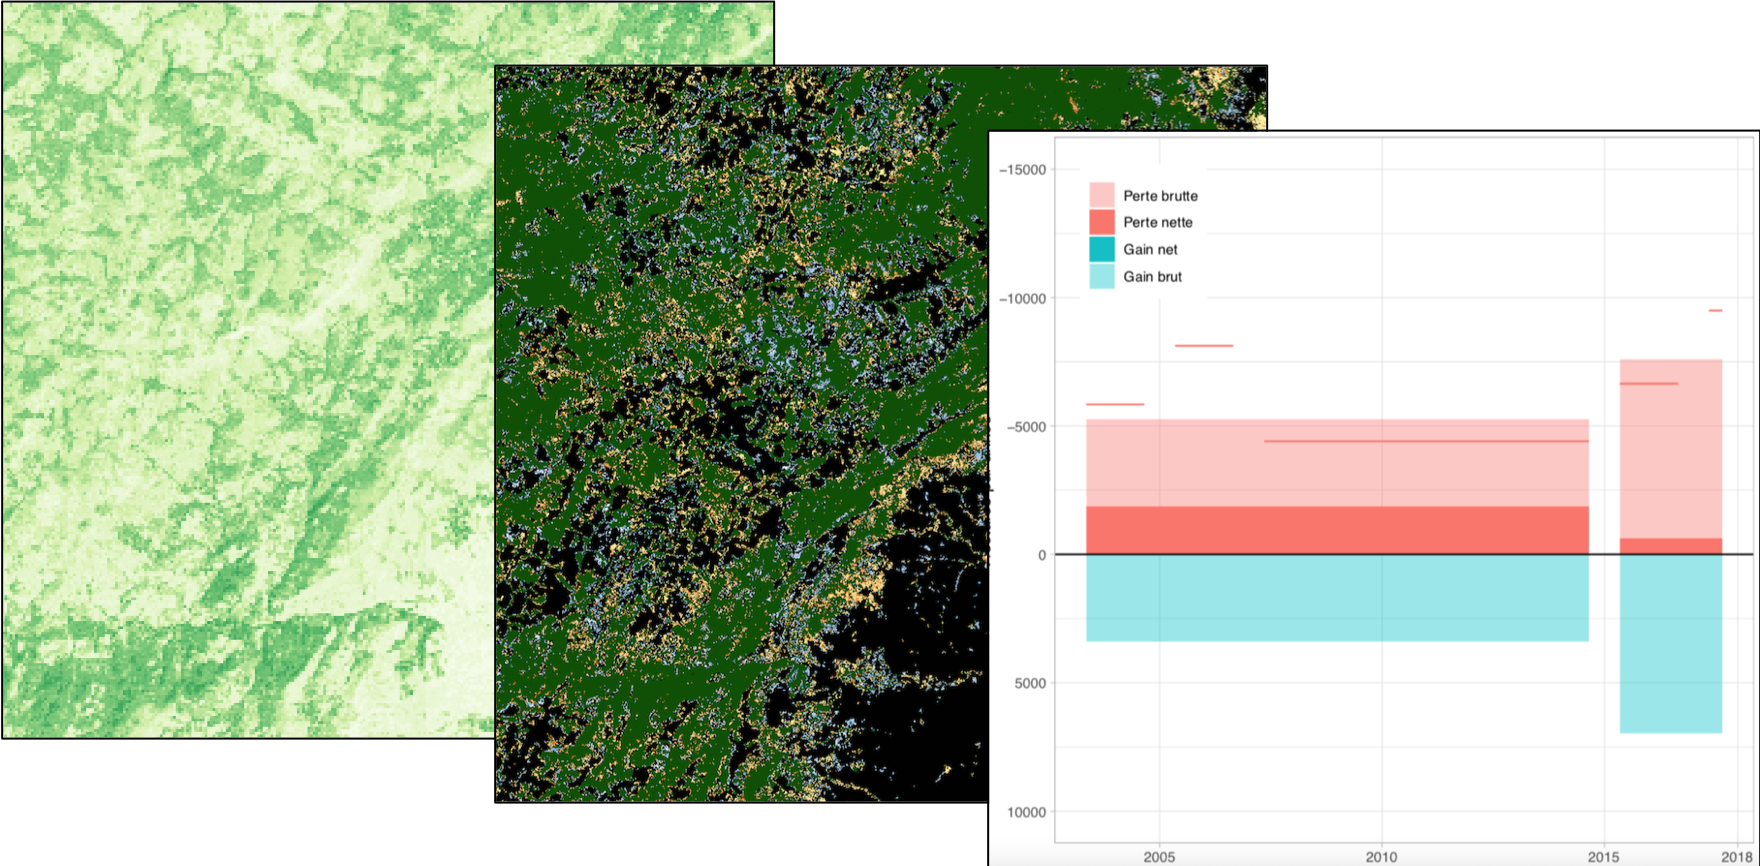
\includegraphics{images/NERF-Togo.png}

\hypertarget{preface}{%
\section*{Préface}\label{preface}}


Ce manuel de référence à comme objectif de décrire le fonctionnement du \textbf{Système National de Surveillance des Forêts au Togo (SNSF)}. Les éléments traités sont les arrangements instutitionelles, l'implémentation de l'Inventaires Forestier National (IFN) et de Système Surveillance Terrestres par Satellite (SSTS) et l'approche technique pour en sortir les informations nécessaires pour le Niveau de Référence pour les Forêts du Togo (NRF) ainsi que pour le Monitoring, Reporting et Verification (MRV) dans le cadre de l'engagement du Togo pour le REDD+.

La partie \protect\hyperlink{NRF-MRV}{Analyses NRF/MRV} décrit en détail les outils utilisés pour établir et le \textbf{Niveau de Référence pour les Forêts du Togo 1.0}, soumis au sécrétariat CCNUCC en Janvier 2020 et pour mettre à jour les analyses dans le cadre d'une surveillance de la biomasse forestier continue dans le cadre du Monitoring, Reporting et Verification pour la REDD+. Les résultats de ces analyses sont publiés ailleurs (liens sur les rapports sur le site CCNUCC et géoportail).

En cas de questions, veuillez contacter la \href{http://www.reddtogo.tg/index.php/contacts}{Coordination nationale REDD+ du Togo}

\hypertarget{introduction}{%
\section{Introduction}\label{introduction}}

L'objectif du Système National de Surveillance des Forêts (SNSF) est d'évaluer régulièrement \textbf{l'état des forêts togolaises et leur évolution}. Dans le \href{http://faolex.fao.org/docs/pdf/tog85011.pdf}{code forestier du Togo}, la forêt est définie comme:

\begin{quote}
un espace occupant une superficie de plus de 0,5 hectare avec des arbres atteignant une hauteur supérieure à 5 mètres et un couvert arboré de plus de 10 pour cent, ou avec des arbres capables d'atteindre ces seuils in situ.
\end{quote}

Pour l'évaluation du développement des zones forestières, le SNSF distingue entre \textbf{terres forestières} avec un couvert des houppiers \(geq\) 30\% et les \textbf{terres boisées} avec un couvert des houppiers entre 10\% -- 30\%.

\begin{rmdtodo}
Actuellement, sur base des images Landsat, le SNSF enregistre que
l'évolution des terres forestiers avec une couverture des houppiers
\(geq\) 30\%. Des données satellitaires de plus haute resolution seront
nécessaires pour évaluer également les terres boisées.
\end{rmdtodo}

Le SNSF combine les données recueillies sur le terrain avec les données des images satellites pour fournir des informations sur lévolution du l'ensemble des forêts dans le pays. Comme illustré dans l'image au-dessous et décrit dans les sections suivantes, \textbf{le SNSF consiste de trois pilliers principaux:}

\begin{itemize}
\item
  Le \protect\hyperlink{IFN}{\textbf{Inventaire Forestier National (IFN)}} recueille des informations détaillées sur l'état des forêts sur un nombre limité de placettes d'échantillonnage permanentes sur le terrain.
\item
  Au moyen du \protect\hyperlink{SSTS}{\textbf{Système de Surveillance Terrestre par Satellite (SSTS)}}, des informations sur la couverture et l'utilisation des sols sont recueillies sur un grand nombre de parcelles d'échantillonnage à partir d'images satellites. Avec l'aide du SSTS, les informations sur l'IFN peuvent être extrapolées à l'ensemble du pays.
\item
  Le \protect\hyperlink{NRF-MRV}{\textbf{Niveau de Référence des Forêts (NRF) ainsi que le Monitoring, Reporting et Vérification (MRV)}} des changements dans le réservoirs carbone forestiersest une applications du SNSF pour informer la communauté internationale sur l'engagement du Togo dans le cadre du mécanisme REDD+. Dans ce cadre, les données de la IFN sont utilisées pour déterminer le stockage du carbone dans la biomasse des arbres, tandis que les données de la SSTS sont utilisées pour déterminer le changement de la superficie forestière. Ensemble, cela se traduit par les pertes de carbone dues à la déforestation et la séquestration du carbone provenant du reboisement.
\end{itemize}

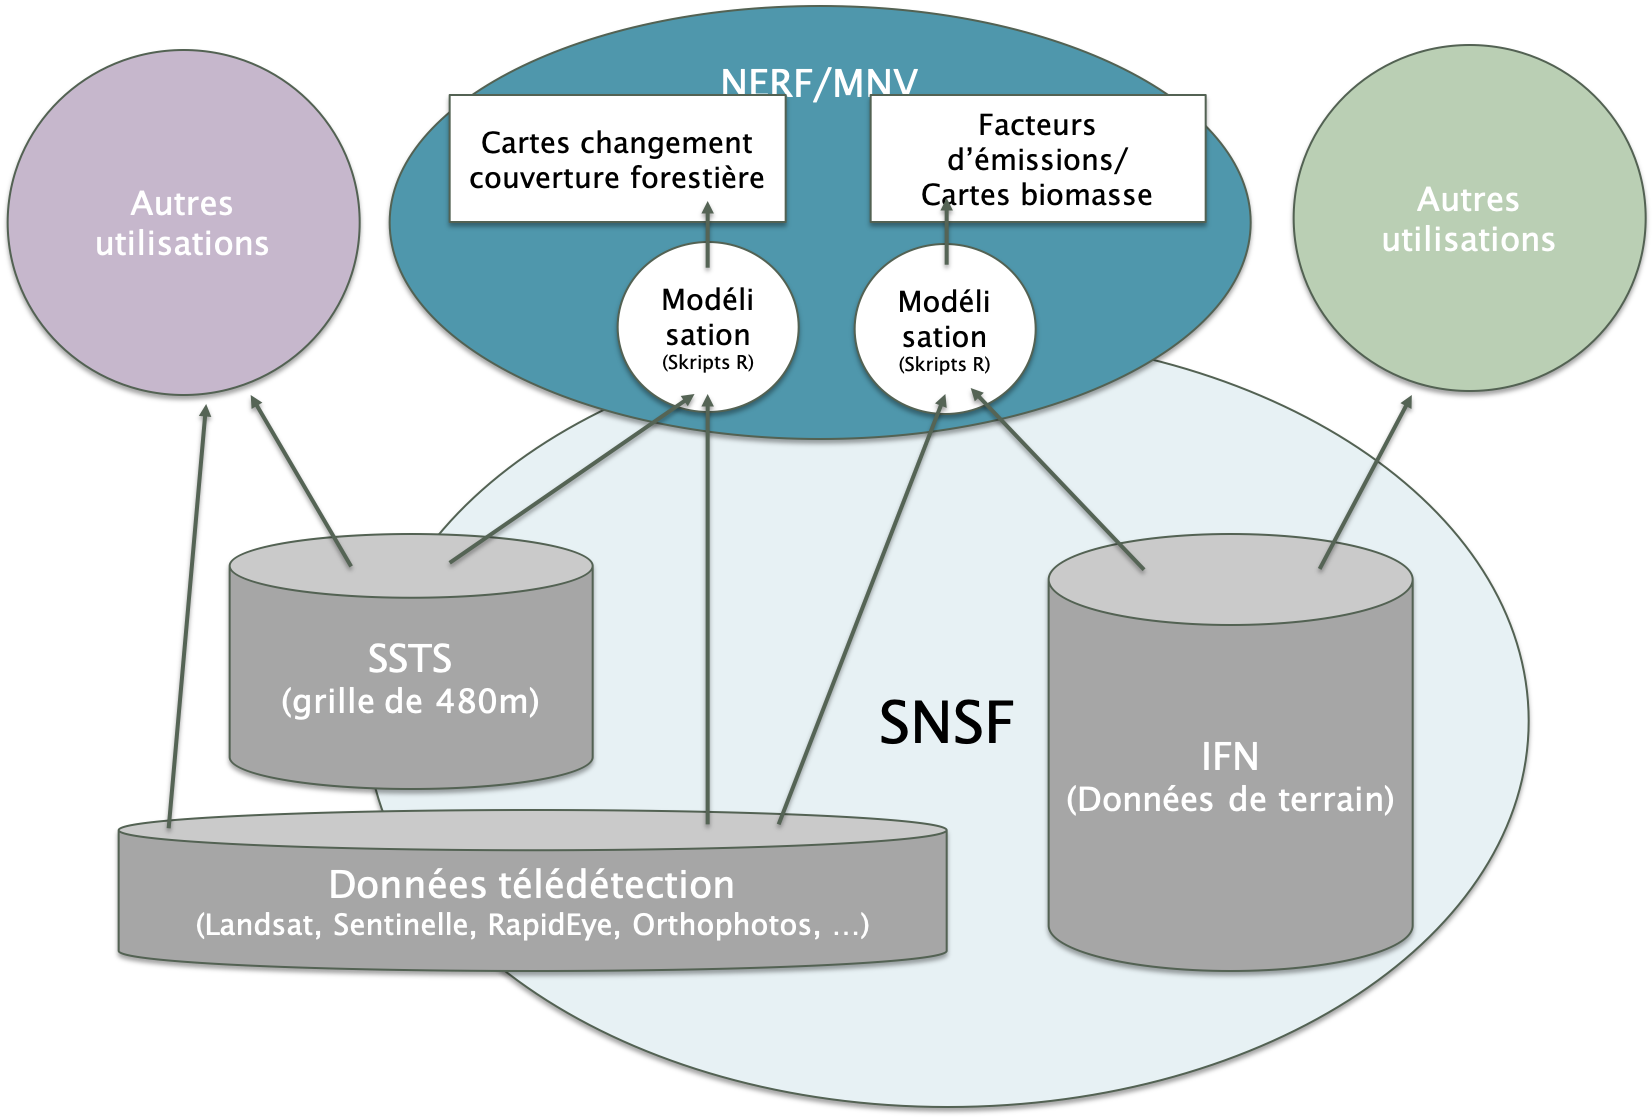
\includegraphics{images/SNSF-Schema.png}

\begin{rmdtodo}
\textbf{En future, d'autres sources de données pourraient être intégrées
au SNSF}, telles que

\begin{itemize}
\tightlist
\item
  le carbone organique du sol (prévu à rélever dans l'IFN-2)
\item
  feux de brousse (base de données SANGE)
\item
  dégradation des forêts (utilisation des images de haute résolution
  Sentinel-2)
\item
  droits fonciers
\item
  plantations
\item
  exploitation du bois
\item
  \ldots{}
\end{itemize}

Pour l'avenir, il est également prévu d'impliquer la population locale
dans la surveillance des forêts, par exemple en signalant les activités
irrégulières à l'aide d'une application pour smartphone.
\end{rmdtodo}

\printindex

\end{document}
